\documentclass[a4paper]{article}
\usepackage{cheatsheet}
\usepackage{multicol}
\usepackage{multirow}
\usepackage{makecell}
\usepackage{enumitem}
\usepackage{tabularx}
\usepackage{amsmath}
\usepackage{amssymb}
\usepackage{ulem}
\usepackage{pdfpages}
\usepackage{graphicx}


\setenumerate[1]{itemsep=0pt,partopsep=0pt,parsep=\parskip,topsep=0pt, leftmargin=*}
\setitemize[1]{itemsep=0pt,partopsep=0pt,parsep=\parskip,topsep=0pt, leftmargin=*}
\setitemize[2]{itemsep=0pt,partopsep=0pt,parsep=\parskip,topsep=0pt, leftmargin=*}
\setdescription{itemsep=0pt,partopsep=0pt,parsep=\parskip,topsep=0pt, leftmargin=*}

\begin{document}

\begin{multicols}{3}

\begin{cheatsheetblock}{Relational Data Model}
    \begin{tabularx}{\linewidth}{|X|X|X|}
        \hline
        \textbf{Formal} & \textbf{Informal} & \textbf{Denoted}                             \\
        \hline
        Relation Schema & Table Define      & $R(A_1, A_2,\allowbreak\dots, A_n)$          \\
        \hline
        \makecell[l]{Relation                                                              \\relation state\\relation instance}
                        & Table             & $r(R) := \{t_1, t_2\allowbreak,\dots, t_m\}$ \\
        \hline
        Tuple           & Row               & $t_1:=t(A_1)$                                \\
        \hline
        Attribute       & Column            & $A_1$                                        \\
        \hline
        Domain          & Data Type         & $D:=\mathrm{dom}(A_i)$                       \\
        \hline
    \end{tabularx}
    \begin{itemize}[topsep=0pt, noitemsep, ]
        \item $t_1 \in r(R) \subseteq R(A_1, \dots, A_n)$
        \item $t_1 \in \mathrm{dom}(A_1) \times \dots \times \mathrm{dom}(A_n)$
        \item $r(R) \subseteq \mathrm{dom}(A_1) \times \dots \times \mathrm{dom}(A_n)$
        \item $R(A_1, \dots, A_n) \equiv \mathrm{dom}(A_1) \times \dots \times \mathrm{dom}(A_n)$
    \end{itemize}
\end{cheatsheetblock}

\begin{cheatsheetblock}{Keys}
    \begin{itemize}
        \item superkey: uniquely identifes any tuple in $r(R)$.
        \item candidate key: no proper subset of $K$ is a superkey.
        \item primary key: chosen from the candidate keys.
        \item prime attribute: attribute occurring in a candidate key.
    \end{itemize}
\end{cheatsheetblock}

\begin{cheatsheetblock}{ Functional Dependencies}
    Notation:
    \begin{itemize}
        \item $X \rightarrow Y$ \hfill FD: Dependent to Determinant
        \item $\Sigma \models X \rightarrow Y$, \hfill FD set imply FD.
        \item $\Sigma^*$, \hfill all FD implied by $\Sigma$.
        \item $X^+$, \hfill closure, all attributes $X \rightarrow$.
    \end{itemize}
    Rules (Armstrong’s inference rules)
    \begin{itemize}
        \item $X Y \rightarrow Y$ \hfill Reflexive rule
        \item $\{X \rightarrow Y\} \models X Z \rightarrow Y Z$ \hfill Augmentation rule
        \item $\{X \rightarrow Y, Y \rightarrow Z\} \models X \rightarrow Z$ \hfill Transitive rule
        \item Union rule, Decomposition rule
    \end{itemize}
\end{cheatsheetblock}

\begin{cheatsheetblock}{FD Algorithm}
    check $\Sigma \models X \rightarrow W$ \hfill compute $X^+$ by repeatedly apply FD in $\Sigma$.
\end{cheatsheetblock}

\begin{cheatsheetblock}{Minimal Cover}
    \begin{enumerate}
        \item Dependent R side: $X \rightarrow\left\{A_1, A_2\right\} \implies X \rightarrow A_1, X \rightarrow A_2$
        \item Determinant L side: replace $XY \rightarrow \left\{A\right\}$ to $X \rightarrow \left\{A\right\}$, if ok.
        \item Remove redundant FD
    \end{enumerate}
\end{cheatsheetblock}

\begin{cheatsheetblock}{Find Keys}
    \begin{enumerate}
        \item compute all $X^+$
        \item $X^+ = R$, X is a superkey
        \item no proper subset in $X^+$ is a superkey, X is a (candidate) key
    \end{enumerate}

    \textbf{trick}
    start with attribute never appear on the R side. Must be a key attribute.
\end{cheatsheetblock}

\begin{cheatsheetblock}{BCNF (Boyce-Codd Normal Form)}
    \textbf{def}: All non-trivial FDs, left side is a superkey.

    \textbf{Algorithm} start with $S = \left\{R^\prime\right\}$ and iter
    \begin{enumerate}
        \item find FD violations in $R \in S$
        \item replace the $R$ by $XY$ and $R-Y$
    \end{enumerate}
\end{cheatsheetblock}

\begin{cheatsheetblock}{3NF (3rd Normal Form)}
    \textbf{def}: All non-trivial FDs, left side is a superkey or right side is prime attribute.

    \textbf{Algorithm} start with $S = \varnothing$ and minimal cover $\Sigma^\prime$.
    \begin{enumerate}
        \item group by L-side. \hfill $X \rightarrow A_1, A_2$
        \item combine attributes within group \hfill $R = \left\{X, A_1, A_2\right\}$
        \item remove redundant FDs \hfill \sout{$R_1 = \left\{X, A_1\right\}$}, $R_2 = \left\{X, A_1, A_2\right\}$
        \item if $S$ contain no superkey, add one from $R$. \hfill $S = \left\{R_2, R_0\right\}$
        \item project FDs onto each schema
    \end{enumerate}
\end{cheatsheetblock}

\begin{cheatsheetblock}{Relational Algebra}
    \begin{itemize}
        \item $\sigma_{\text {Sex}\neq\text {`M'}} (\text{Employee})$ \hfill SELECT * \textbf{WHERE sex != `M'}
              \subitem selection, commutative
        \item $\pi_{\text {Name}, \text {Id}} (\text {Employee})$ \hfill SELECT \textbf{DISTINCT name, Id}
              \subitem project, not commutative
        \item $R_1 \cup R_2$ \hfill UNION (no ALL)
        \item $R_1 \cap R_2$ \hfill INTERSECT
        \item $R_1 - R_2$ \hfill EXCEPT
        \item $R_1 \times R_2$ \hfill FROM R1, R2
              \subitem cross product
        \item $R_1 \bowtie_{Id = Sid} R_2$ \hfill JOIN ON R1.Id = R2.Sid
              \subitem $\equiv \sigma_{Id = Sid} (R_1 \times R_2)$
        \item $\rho_{R^{\prime}\left(A_1, \dots, A_n\right)}(R)$ \hfill (SELECT R1 \textbf{AS A1}, \dots) \textbf{AS $R^{\prime}$}
              \subitem rename, allow only $\left(A_1, \dots, A_n\right)$ or only $R^{\prime}$.
    \end{itemize}
    a complete set: $\left\{\sigma, \pi, \rho, \cup, -, \times\right\}$
\end{cheatsheetblock}

\begin{cheatsheetblock} {Opt Heuristic Rules}
    \begin{itemize}
        \item $\sigma_{\varphi}\left(\sigma_\psi(R)\right) \equiv \sigma_{\varphi \wedge \psi}(R)$
        \item $\pi_X\left(\pi_Y(R)\right) \equiv \pi_X(R)$ if $X \subseteq Y$
        \item $\sigma_{\varphi}\left(R_1 \times R_2\right) \equiv R_1 \bowtie_{\varphi} R_2$
        \item $\sigma_{\varphi_1}\left(R_1 \bowtie_{\varphi_2} R_2\right) \equiv R_2 \bowtie_{\varphi_1 \wedge \varphi_2} R_1$
        \item $\sigma_{\varphi}\left(R_1 \bowtie R_2\right) \equiv \sigma_{\varphi}\left(R_1\right) \bowtie R_2$, if $\varphi$ solely on $R_1$
        \item $\sigma_{\varphi_1 \wedge \varphi_2}\left(R_1 \bowtie R_2\right) \equiv \sigma_{\varphi_1}\left(R_1\right) \bowtie \sigma_{\varphi_2}\left(R_2\right)$
              if $\varphi_1$ solely on $R_1$ and $\varphi_2$ on $R_2$. $\bowtie$ can be $\times$
        \item $\pi_X\left(R_1 \bowtie R_2\right) \equiv \pi_{X_1}\left(R_1\right) \bowtie \pi_{X_2}\left(R_2\right)$ If the join condition involves only attributes in $X$.
        \item $\pi_X\left(R_1 \bowtie R_2\right) \equiv \pi_X\left(\pi_{X_1}\left(R_1\right) \bowtie \pi_{X_2}\left(R_2\right)\right)$ If the join condition involves NOT only attributes in $X$.
    \end{itemize}
\end{cheatsheetblock}

\begin{cheatsheetblock} {Query Processing}
    \begin{itemize}
        \item Parser: checks the name, type, permission.
        \item Translator: decomposed query $\rightarrow$ query blocks; \\ translated into a Relational Algebra expression.
        \item Optimiser: optimisation
        \item Evaluation engine: evaluate the query execution plan
    \end{itemize}
\end{cheatsheetblock}

\begin{cheatsheetblock} {Optimisation}
    \begin{itemize}
        \item Semantic query optimisation: using constraints.
        \item Rule-based query optimisation.
              \begin{itemize}
                  \item Push-down selection, projection; Re-ordering joins
              \end{itemize}
        \item Cost-based query optimisation: estimate cost among plans, choose most cost-effective plan
    \end{itemize}
\end{cheatsheetblock}

\begin{cheatsheetblock}{(Enhanced) Entity-Relationship (EER) Model}
    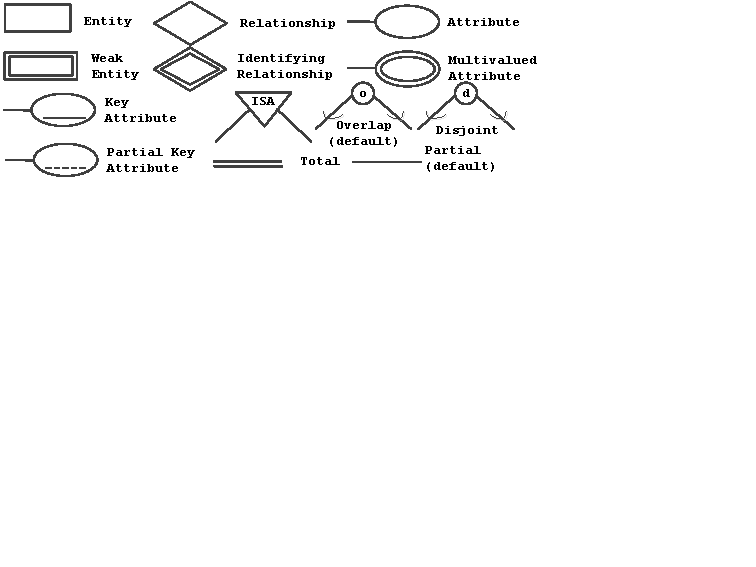
\includegraphics[width=\linewidth, page=1]{pic/EER.pdf}
\end{cheatsheetblock}

\begin{cheatsheetblock}{Database Transactions}
    \textbf{ACID}: Atomicity, Consistency, Isolation, Durability.

    C - defined business rules; I - concurrent; D - persist.

    \textbf{Problems}
    \begin{itemize}
        \item Lost Update: R1R2,\textbf{W1W2},C1C2 \hfill S?
        \item Dirty Read: R1W1R2,\textbf{A1}(abort),W2C2 \hfill CRS
        \item Unrepeated read: R1,R2\textbf{W2}C2,R1 \hfill RS
        \item Phantom read: R1,\textbf{W2}C2,R1 \hfill S
    \end{itemize}
    
    \textbf{Isolation Level}: Read [U]ncommitted, Read [C]ommitted, Repeatable [R]eads, [S]erializable
\end{cheatsheetblock}

\begin{cheatsheetblock}{Database Security}
    \textbf{Threats}: Lost of confidentiality, integrity, availability.

    \textbf{Control}: Access, Inference, Flow, Data encryption.

    \textbf{Access}: Discretionary (privileges), Mandatory, Role-based.

    Privileges: \hfill GRANT operations ON object TO users [OPT]
    
    Revoking: \hfill REVOKE operations ON object FROM users

    view: \hfill CREATE VIEW name AS SELECT \dots

    Mandatorys: top secret, secret, confidential, unclassified

\end{cheatsheetblock}

\begin{cheatsheetblock}{SQL Injection}
    \dots WHERE ... password=`\underline{p' OR `x'=`x}';

    \dots WHERE ... password=`\underline{p'; DROP TABLE users; --;}';

    Solution: Parameterized queries (placeholder), Input validation (escape)
\end{cheatsheetblock}

\begin{cheatsheetblock}{Database Management System}
    For: defining, constructing(store), manipulating, sharing.

    ANSI/SPARC Architecture: External, Conceptual/logical, Internal.

    Logical Data Independence; Physical Data Independence.
\end{cheatsheetblock}

\begin{cheatsheetblock}{Update Anomalies}
    Insertion, Deletion, Modifcation.
\end{cheatsheetblock}

\end{multicols}

\end{document}
